\chapter[Referencial Teórico]{Referencial Teórico}
Neste capítulo, são apresentadas as bases teóricas para o desenvolvimento do \textit{framework}. O capítulo está organizado em seções. Na seção 2.1, faz-se referência ao contexto de Verificação e Validação de Software. Na seção 2.2, aborda-se uma temática mais específica da qualidade de software, os testes. Traz a motivação para fazê-los, bem como uma descrição sobre os níveis de testes e as vantagens e estratégias de automatizá-los. Na seção 2.3, dicuti-se sobre \textit{frameworks}, sua definição, motivação, vantagens e desvantagens e classificação. Na seção 2.4, explana-se sobre a geração de testes e técnicas de implementá-la.

\section{Verificação e Validação de Software}
Software é uma atividade que requer um processo com o envolvimento de diversas atividades e diferentes pessoas. Essa característica acaba por favorecer - mesmo não sendo desejado - a inserção de defeitos no produto final \cite{trodo2009}. Além disso, há o risco de se produzir algo que não foi solicitado, devido ao mau entendimento dos requisitos\cite{barbosaEtAl2009}. Esse conjunto de fatores fez surgir uma maior preocupação em relação à qualidade de software e, inclusive nesse contexto, é que há o advento da Engenharia de Software, com o objetivo de produzir software com qualidade \cite{buenoCampelo2013}.
\par
\indent Tendo em vista o cuidado com o nível dos software, surge a necessidade de conceituar qualidade no que tange esse assunto. Essa definição é díficil, pois qualidade é um conceito abstrato. Em essência, a qualidade esta ligada à possibilidade de medir determinado atributo e comparar o resultado com padrões já conhecidos \cite{buenoCampelo2013}. No âmbito de software, há também o conceito de métricas. Elas são utilizadas para dar visibilidade de determinadas características do produto, de forma a demonstrar o tamanho, o esforço e a complexidade do software em construção, dentre outros atributos \cite{abreu2011}.
\par
\indent Tendo isso em vista, observa-se que, no que se refere ao software, tem-se como caracterizar a qualidade em dois tipos, na medida em que há características mensuráveis tanto no projeto quanto no produto. São eles: qualidade de projeto e qualidade de conformidade. O primeiro diz respeito aos requisitos, especificações e arquitetura. Enquanto que o segundo, foca na implementação e sua conformidade com o que foi especificado \cite{buenoCampelo2013}.
\par
\indent A qualidade de software está ligada à atividade de verificação e validação de software \cite{buenoCampelo2013}. A qualidade de software é uma atividade que pertence ao ambiente de gerência, enquanto que a verificação e validação de software é uma prática mais técnica e enquadra-se no desenvolvimento do produto \cite{buenoCampelo2013}. Segundo \citeonline{sommerville2007}, verificação e validação de software é o processo que certifica que o produto em desenvolvimento atende às especificações esperadas pelo cliente. Essa atividade deve permear todo o processo de produção do software, de forma a garantir que o produto respeita o especificado desde o início. Essa prática evita que a identificação de defeitos seja percebida apenas ao final do desenvolvimento, o que aumentaria os custos do projeto.
\par
\indent Verificação e validação são dois conceitos muitas vezes confundidos. Verificação de software busca analisar se o produto está em conformidade com o que foi especificado. É nessa atividade que se observa o quão próximo está o produto das especificações dos requisitos, sejam eles funcionais ou não funcionais \cite{sommerville2007}. A validação de software objetiva garantir que o software é o que o cliente solicitou \cite{sommerville2007}. Assim, pode-se conceituar verificação e validação da seguinte forma:
\begin{itemize}
\item Verificação: análise sobre o produto, afim de observar se o produto está sendo feito de maneira certa.
\item Validação: avalia se o produto em construção é o correto em relação às expectativas do cliente.
\end{itemize}
\par
\indent O processo de verificação e validação é responsável por gerar a certeza de que o software está adequado ao que foi pedido \cite{sommerville2007}. Para essa tarefa, a verificação e validação utiliza-se de duas abordagens, principalmente: inspeções de software e testes de software. Inspeção de software é um processo estático, o que significa que não há a necessidade do sistema estar em funcionamento. Essa atividade é baseada em revisões, com o intuito de identificar erros e omissões. Toda forma de representação do software é passível de uma inspeção (especificações de requisitos, arquitetura, dentre outros). No entanto, o código-fonte é um foco \cite{sommerville2007}. Teste de software é um processo dinâmico, o que exige o funcionamento do software enquanto ele ocorre. Objetiva a demonstração de que o software esta conforme os requisitos, a revelação de falhas ou defeitos no software \cite{sommerville2007} e a prevenção de novas inserções de defeitos \cite{burkeCoyner2003}.

\section{Testes de Software}
Testes de software representam uma atividade que compõe o processo de verificação e validação de software. É uma das técnicas mais utilizadas no âmbito de garantia de confiabilidade de software. Em linhas gerais, é um trabalho de abordagem dinâmica sobre o código-fonte. Isso significa que há a exigência do funcionamento do software para que possa ser realizada essa atividade \cite{barbosaEtAl2009}. Essa análise dinâmica abre a possiblidade de identificação de defeitos no código-fonte, bem como a prevenção de inserções de novos defeitos. A produção de testes de software fornece, ainda, impulso para atividades de refatoração, manutenção e medição do software \cite{barbosaEtAl2009}.
\par
\indent Os testes podem ser classificados em \textbf{níveis}. Essa divisão refere-se ao nível de abstração dos testes. Quanto mais próximo do código, menos abstrato o nível do teste \cite{sommerville2007}. Os testes de software são divididos da seguinte forma, em ordem descrescente de abstração:
\begin{description}
\item[Testes de aceitação:] são testes cuja finalidade é garantir que as especificações do software foram implementadas, de forma a corresponder às necessidades do usuário final. Em essência, é um teste de validação do software. \cite{sommerville2007}.
\item[Testes de sistema:] tipo de teste que visa observar se o sistema funciona por completo. Diferentemente dos testes aceitação, seu foco não é a experiência do usuário, mas se o sistema é seguro, responde às requisições \cite{sommerville2007}.
\item[Testes de integração:] fazem a análise e a identificação de defeitos relacionados à integração de dois ou mais componentes do software. Normalmente, visam as \textit{interfaces} que interagem com esses componentes \cite{sommerville2007}.
\item[Testes de unidade:] é o processo de teste de partes específicas do código-fonte. Busca a seleção de partes pequenas, mas de valor significativo, do código para fazer o teste. Normalmente, os métodos (ou funções-membro) são considerados unidades. Essa análise possibilita a verificação do código, de forma a identificar defeitos e mitigá-los \cite{sommerville2007}.
\end{description}
\par
\indent Os testes podem também ser classificados como: testes caixa-preta e testes caixa-branca \cite{barbosaEtAl2009}.

\subsection{Testes Caixa-preta}
Testes caixa-preta, também conhecidos como testes baseados em especificações. Esses testes visam à avaliação do produto em relação aos requisitos funcionais e não funcionais. São caracterizados por realizarem análises a partir de documentação e do software em funcionamento, sem necessidade de averiguação do código-fonte \cite{barbosaEtAl2009}.

\begin{figure}[h]
  \centering
    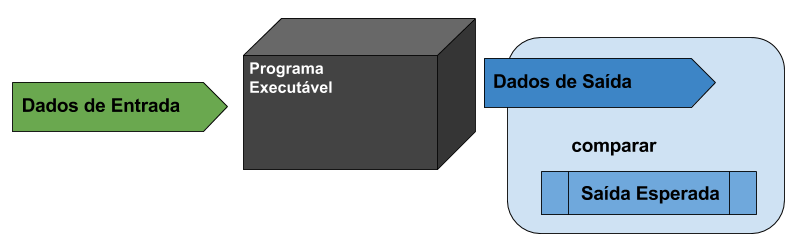
\includegraphics[width=0.8\textwidth]{figuras/test_black_box.png}
    \caption{Diagrama Representativo de Testes Caixa Preta}
    \label{test_black_box}
\end{figure}

A Figura \ref{test_black_box} representa um esquemático do funcionamento de um teste caixa-preta: utiliza-se dados de entrada no software e observa-se a correspondência, ou não, com as expectativas.
\par
\indent Ao fazer uso de testes caixa preta, os testes sob o ponto de vista do usuário são desenvolvidos, o que auxilia na observação de falhas nas especificações. Além disso, permite que os casos de teste possam ser produzidos assim que as especificações estiverem prontas \cite{stf2010}. Essa abordagem de testes também possui pontos negativos, como a pequena quantidade de entradas que podem ser inseridas para testar o produto. Sem especificações claras, produzir bons casos de testes caixa-preta torna-se uma tarefa difícil \cite{stf2010}.
\par
\indent A seguir são demonstradas algumas técnicas para a derivação de Testes de caixa-preta.

\subsubsection{Técnicas de Derivação de Casos de Teste Caixa-preta}
Testes caixa-preta não são o foco deste trabalho. Dessa forma, apenas um \textit{overview} das técnicas para essa abordagem de testes será considerado. Para a concepção de casos de testes caixa-preta, há algumas técnicas utilizadas como guias. São elas: \textbf{classes de equivalência}, \textbf{análise de valores limite} e \textbf{grafo de causa e efeito}.

\begin{description}
\item[Classes de equivalência:] visa a identificação de agrupamentos de casos de testes que cubram diferentes classes de erros. Essa estratégia permite a redução do número de testes que serão produzidos, diminuindo os custos. A técnica de classes de equivalência divide as entradas do domínio do software em classes. Essas classes devem ser derivadas a partir de um valor significativo para o domínio \cite{williams2006}.
\item[Análise de valores limite:] um ponto crítico, e já observado por especialistas, é que grande parte dos defeitos no código são inseridos nos limites de uma classe de equivalência. Isso permite a conclusão de que o principal foco no caso de teste deve ser sobre os valores limites. Entende-se como \textbf{limite} um valor que esteja imediatamente próximo ao valor de entrada significativo que divide o domínio em classes de equivalência. Sendo assim, num contexto onde o valor significativo, para separar duas classes de equivalência, seja 50, possíveis valores limite seriam 49 e 51 \cite{williams2006}.
\item[Grafo de causa e efeito:] é uma representação visual das relações entre as entradas e saídas. Permite a observação lógico-combinatória das especificações do programa. É uma representação semelhante a circuitos lógicos. Sua principal vantagem é a visualização que se dá, permitindo identificar casos de teste muito facilmente. No entanto, quando a rede fica muito grande e complexa, passa a ser considerado o uso de outras técnicas \cite{barbosaEtAl2009}.
\end{description}


\subsection{Testes Caixa-branca}
Testes de caixa-branca, também referenciados como testes baseados em programa, almejam a avaliação do produto por meio da execução do código-fonte. Isso possibilita o exercício do software em busca de defeitos para serem corrigidos. Para que ocorra a dinâmica de testes de caixa-branca, os casos de testes que englobem cenários significativos são selecionados \cite{barbosaEtAl2009}.
\par
\indent Algumas vantagens de teste de caixa-branca podem ser listadas: pode-se dar início ao desenvolvimento de testes desde o começo da codificação, na medida em que a interação com interfaces não é necessária. Além disso, é um tipo de teste capaz de cobrir mais caminhos, pois tem um alcance mais profundo no software. Com relação aos pontos negativos, cita-se a necessidade de programadores para efetuar os testes de caixa-branca \cite{barbosaEtAl2009}.
\par
\indent A seguir são demonstradas algumas técnicas para a derivação de Testes de caixa-preta.

\subsubsection{Técnicas de Derivação de Casos de Teste Caixa-branca}
Os testes de caixa-branca são utilizados objetivando que todos os caminhos independentes possam ser percorridos e testados. Algumas técnicas para derivação de casos de teste são utilizadas, com o intuito de garantir que todos os caminhos tenham sido percorridos, pelo menos um vez, e assegurar uma quantidade de teste exclusivamente necessária. São elas: \textbf{Cobertura de Comandos}, \textbf{Cobertura de Decisão}, \textbf{Cobertura de Condição} e \textbf{Cobertura de Decisão-condição} \cite{istqb2014}.

\begin{description}
\item[Cobertura de comandos:] também conhecida como cobertura de linha ou cobertura de segmento. Tem por propósito a execução de todos os comandos do código, ao menos uma vez. Caracteriza-se por cobrir unicamente as linhas com condição verdadeira, e por permitir a observação dos comandos que, por algum motivo, não estão sendo executados. É considerada uma estrátegia incompleta, pois não permite o teste de condições falsas, muito menos a execução de testes de \textit{loops} de forma a ter certeza de sua condição de término \cite{istqb2014}.
\item[Cobetura de decisão:] semelhante à técnica de cobertura de comando, entretanto, desenhada para que tanto as condições verdadeiras quanto as falsas sejam cobertas pelos casos de teste. Da mesma forma que a cobertura de comando, pode deixar de identificar defeitos, pois cobrir uma linha de código não garante que o comando esteja livre de defeitos. Também é chamada de cobertura de ramificações. \cite{istqb2014}.
\item[Cobertura de condição:] define-se por ser uma estratégia mais sensível aos possíveis caminhos no fluxo de controle. Busca cobrir todos os possíveis valores significativos relativos a uma condição no fluxo \cite{istqb2014}.
\item[Cobertura de decisão-condição:] é uma estratégia que pretende unir as vantagens da cobertura de decisão e de condição \cite{istqb2014}.
\end{description}
\par
\indent Utilizando-se de um grafo de fluxo de controle fica mais fácil a visualização e identificação dos caminhos a serem testados \cite{copeland2003}.
\par
\section{Reutilização de Software}
O conceito de reutilização é antigo dentro do domínio da engenharia. Foi utilizado a bastante tempo por culturas antigas, como os egípios (\textit{design} das pirâmides) e os romanos (arcos na construção civil). A engenharia civil utiliza-se do conceito de reutilização de soluções e de componentes \cite{sutcliffe2002}. O uso do desenvolvimento baseado em componentes também está presente no universo de software, entretanto, num cenário menos consolidado \cite{sutcliffe2002}.
\par
\indent \textbf{Reutilização} é o uso de conceitos, ou objetos, previamente adquiridos, mas em um novo contexto \cite{sutcliffe2002}. Tendo isso em vista, entende-se que para alcançar o reutilização há a necessidade de entender o problema e a solução. A partir disso, encapsular em diferentes níveis de abstração, para conseguir extrair conceitos passíveis de serem duplicados e/ou adaptados \cite{sutcliffe2002}.
\par
\indent Portanto, pode-se entender como reutilização de software o desenvolvimento de software a partir de abstrações, sendo estas conceituais ou componentizadas, que já foram utilizadas com sucesso em outros contextos \cite{sutcliffe2002}.

\subsection{\textit{Frameworks}, Biliotecas de Classe e \textit{Design Patterns}}
Durante o desenvolvimento de software, a reutilização de soluções é uma prática bastante comum. Há diversas formas de colocar em prática o reutilização, como por exemplo o uso de \textbf{\textit{frameworks}}, \textbf{bibliotecas} e \textbf{\textit{design patterns}}. Essas formas de reutilização de software, em alguns momentos, podem ser semelhantes, no entanto, são técnicas distintas \cite{barretoJunior2006}.
\par
\indent Os três modos de reutilização de software possuem pontos parecidos, como refletir abstrações, generalizando um domínio de problemas e demonstrando uma solução (\textit{frameworks} e \textit{design pattern}), ou mesmo configurando-se como um conjunto de classes capaz de dar suporte ao desenvolvedor por meio de soluções já pensadas e implementadas (\textit{frameworks} e bibliotecas de classes e/ou funções).
\par
\indent Da mesma forma, há também pontos que diferenciam esses tipos de reutilização de software.
  \begin{figure}[h]
    \centering
    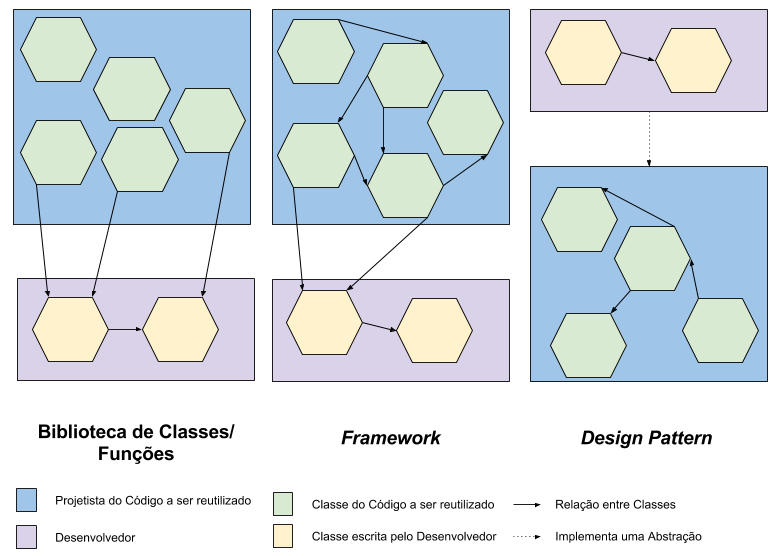
\includegraphics[width=\textwidth]{figuras/bibFrameworkDesignPattern.png}
    \caption{Diferença entre Formas de Reuso de Software}
    \label{fig:bibFrameworkPattern}
  \end{figure}
\par
\indent A Figura \ref{fig:bibFrameworkPattern} esquematiza algumas diferenças, bem como conceitos desses modos de reutilização de software. Como demonstrado na Figura \ref{fig:bibFrameworkPattern}, biliotecas de classes possuem componentes, classes e/ou funções, já prontos, da mesma forma que \textit{frameworks}, entretanto, não há conexão entre eles. São independentes. Em \textit{frameworks}, as classes que o compõe possuem dependências já encravadas por seu projetista, de forma que o modelo de colaboração entre elas já está embutido. Enquanto que ao utilizar-se de uma biblioteca o desenvolvedor deve criar por si só esse modelo de colaboração, caso necessário \cite{barretoJunior2006}.
\par
\indent \textit{Frameworks}, em contra ponto às bibliotecas de classe, são responsáveis por fazer chamadas ao código da aplicação a qual está vinculado. A esse tipo de relação dá-se o nome de \textit{Hollywood Principle} (\textit{"don't call us, we'll call you"}) \cite{sauve2006}.
\par
\indent Outra diferença entre \textit{frameworks}, bibliotecas e \textit{design patterns} é que no  primeiro caso é previsto a justaposição de conhecimento de domínio, são mais especilizados, enquanto que nos demais casos não é previsto isso \cite{sauve2006}.
\par
\indent A Figura \ref{fig:bibFrameworkPattern}f{fig:bibFrameworkPattern} também evidencia algumas diferenças entre os \textit{frameworks} e \textit{design patterns}. \textit{Design patterns} são elementos de software mais abstratos que \textit{frameworks}. Enquanto que \textit{frameworks} concentram a sua característica de reusabilidade a nível de código, os \textit{design patterns} fazem-no exclusivamente a nível de abstração. \textit{Design pattern} é uma ideia, um conceito capaz de abstrair uma solução padrão para um problema já conhecido. \textit{Frameworks} são abstrações de uma solução para um domínio de problema materializadas a nível de código \cite{sauve2006}. Outra diferença a ser citada é que \textit{design pattern} são elementos de software menores que \textit{frameworks}. Normalmente, há uma relação de parte e todo, onde o todo é o \textit{framework} e as partes são os \textit{design patterns}, e essa relação nunca é inversa \cite{sauve2006}.

\subsection{Bibliotecas de Classe}
API, \textit{Application Programming Interface}, é um conjunto particular de regras e especificações que permite a comunicação entre  software \cite{simsek2004}. API's normalmente são vistas como as especificações de como utilizar uma biblioteca de classes, afim de realizar uma tarefa, por meio da interação com a biblioteca \cite{simsek2004}.
\par
\indent Bibliotecas de Classes ou funções, podem ser definidas como sendo a implementação de regras de uma \textbf{API}. Elas disponibilizam um conjunto de funções pré definidas, encarregadas de suprir necessidades comuns de programadores em um dado contexto \cite{simsek2004}. As Bibliotecas são auto-suficientes e abstraem um conjunto de funções comuns a um conceito, como por exemplo, bibliotecas de \textit{strings}, funções matemáticas, manipulação de imagens, algoritmos de ordenação e manipulação de estruturas de dados. Essas características concedem ao programador a facilidade de escrever códigos menores e modularizados, garantindo maior legibilidade e manutenabilidade do código \cite{simsek2004}.
\par
\indent As Bibliotecas podem ser classificadas como \textbf{bibliotecas estáticas} ou \textbf{bibliotecas compartilhadas}. A principal diferença entre essas categorias é em relação a compilação.
\begin{description}
\item[Bibliotecas estáticas:] esse tipo de biblioteca é conectada ao programa que faz uso dela durante a compilação, sem a necessidade de recompilar o aquivo da biblioteca. A principal razão para o uso desse tipo de biblioteca é a redução de tempo de compilação \cite{simsek2004}.
\item[Bibliotecas compartilhadas:] é um tipo de biblioteca que, a partir da ativação do programa, é inserida, o que exige a sua recompilação. O programa não necessariamente inclui código da biblioteca, mas referências às funções contidas nela \cite{simsek2004}.
\end{description}

\subsection{\textit{Design Patterns}}
Uma discussão anterior aos \textit{design patterns} é sobre a arquitetura de software. Há muitas formas de definir arquitetura de sotware. Em uma discussão de alto nível, pode-se dizer que arquitetura de sotware são os formatos e estruturas de uma aplicação de software. Já em uma visão de mais baixo nível, pode-se afirmar que arquitetura de software diz respeito aos módulos da aplicação e suas interconexões, como se relacionam \cite{martin2000}. Um cuidado que projetistas procuram ter com a arquitetura de suas aplicações de sotware é que essas devem ser manuteníveis, livres de falhas críticas, confiáveis e extensíveis \cite{kleinWeiss2009}.

\subsubsection{Princípios de \textit{Design} da Orientação a Objetos}
A partir da necessidade de produzir arquiteturas de software consideradas de qualidade, surgiram alguns princípios considerados essenciais para o \textit{design} de projetos orientados a objetos: \textit{open closed principle}, \textit{liskov substitution principle}, \textit{single responsability principle}, \textit{dependency inversion principle} e \textit{interface segregation principle} \cite{martin2000}.
\begin{description}
\item[\textit{Open closed principle}:] um módulo deve ser aberto para extensões, no entanto, fechado para modificações.
\item[\textit{Liskov substitution principle}:] subclasses deve ser substituíveis por suas classes base.
\item[\textit{Single responsability principle}:] uma classe deve ter apenas uma razão para existir. Cada classe deve lidar apenas com uma responsabilidade.
\item[\textit{Dependency inversion principle}:] deve-se depender de abstrações e não de classes concretas.
\item[\textit{Interface segregation principle}:] é melhor possuir interfaces específicas para os clientes de uma classe, ao invés de uma interface genérica.
\end{description}
\par
\subsubsection{Definição de \textit{Design Pattern}} 
Com o tempo, algumas estruturas utilizadas para solucionar determinados problemas, e que respeitavam os princípios descritas anteriormente, foram sendo repetidas. Essas estruturas são conhecidas como  \textit{design patterns}. \textit{Design pattern}, de uma maneira simplista, são definidos, segundo \citeonline{martin2000}, como \textit{" a well worn and known good solution to
a common problem"}\footnote{\textbf{Tradução:} uma solução bem conhecida e bastante utilizada para problemas comuns.}. Segundo \citeonline{gammaEtAl1994}, \textit{design pattern} é uma solução simples e elegante para um problema específico. São formados por quatro elementos: \textbf{nome}, \textbf{problema associado}, \textbf{a solução} e as \textbf{consequências}.
\begin{description}
\item[Nome:] normalmente é fomado por uma ou duas palavras capazes de invocar tanto o problema a ser atacado e sua solução, bem como as consenquências relativas ao \textit{desgin pattern}. Nomear um \textit{design pattern}, de maneira correta, é importante, na medida em que permite a comunicação fácil entre os desenvolvedores. Permite a referência a um arcabouço de conhecimento e o entendimento entre as partes da conversa de forma simples \cite{martin2000}.
\item[Problema:] é a descrição de quando deve-se aplicar o \textit{design pattern}. Portanto, em qual circunstância deve-se utilizá-lo, explicando o problema e o contexto. É possível ainda listar condições que devem ser observadas para que faça sentido a aplicação do \textit{design pattern} \cite{martin2000}.
\item[Solução:] descreve os elementos que devem ser inseridos no \textit{design}, apontando suas responsabilidades, estruturas e relacionamentos. É importante ressaltar que a solução não deve descrever em detalhes a implementação, e sim a abstração, o conceito por trás da solução. Isso se deve ao fato de que a solução pode ser aplicada a diferentes situações, variando inclusive a linguagem de programação a ser utilizada \cite{martin2000}.
\item[Consequência:] são os resultados da aplicação do \textit{design pattern} ao projeto. Isso envolve a descrição dos benefícios e e os custos do uso do padrão. Demonstra os impactos à flexibilidade, extensibilidade do sistema e tantas outras possíveis características. Tudo deve ser listado para melhorar o entendimento do padrão \cite{martin2000}.
\end{description}
\par
\subsubsection{Classificação dos \textit{Design Patterns}}
A classificação dos \textit{design patterns} vem da necessidade de organizá-los. Além disso, o entendimento do contexto associado a cada uma deles torna-se mais evidente a partir da classificação \cite{gammaEtAl1994}. Como este tema não é escopo desse trabalho, será abordada uma visão geral sobre a classificação dos \textit{design patterns}, sem muitos detalhes. Os \textit{design patterns} podem ser classificados entre: \textbf{padrões criacionais}, \textbf{padrões estruturais} e \textbf{padrões comportamentais}:
\subsubsubsection{Padrões Criacionais}
Esse tipo de \textit{design pattern} objetiva a abstração do processo de instantiação de objetos, permitindo o desenvolvimento de um sistema independente de criação, composição e representação \cite{gammaEtAl1994}.
\par
\indent Esse tipo de padrão viabiliza que o próprio programa decida quais os objetos devem ser criados, para cada caso que surja, adequando-se à situação. Evita determinados problemas que aparecem no método tradicional de criação, por meio de um controle maior dessa ação. Os padrões criacionais possuem duas características marcantes: encapsular o conhecimento sobre as classes concretas utilizadas pelo sistema e esconder como essas instâncias de classes concretas são criadas e combinadas \cite{gammaEtAl1994}.
\subsubsubsection{Padrões Estruturais}
\par
\indent Concentra-se em como classes e objetos são compostos para que possam formar e suportar grandes estruturas. É comum o uso de \textbf{herança} para compor implementações utilizando esses padrões \cite{gammaEtAl1994}.
\par
\indent Descrevem formas de compor objetos, afim de adicionar flexibilidade à composição dos objetos, por meio da capacidade de alterá-la em tempo de execução \cite{gammaEtAl1994}.
\subsubsubsection{Padrões Comportamentais}
Os padrões comportamentais tem por intuito lidar com a comunicação entre objetos e as classes, e qual o comportamento obtido por meio dessa comunicação. Esse padrões fazem uso de complexos fluxos de controle efetuados em tempo de execução. Permite que o desenvolvedor não perca o foco de como interconectar os objetos, na medida em que os \textit{design patterns} concentram-se no fluxo de controle a eles associado \cite{gammaEtAl1994}.
\par
\indent Muitos dos padrões comportamentais utilizam \textbf{composições}, ao invés de herança. Em muitos casos, é possível observar a cooperação entre objetos para o desenvolvimento de uma atividade que, sozinhos, seriam incapazes de fazê-lo \cite{gammaEtAl1994}.

\subsection{\textit{Frameworks}}
\textit{Frameworks} podem ser definidos como uma forma de reutilização de software. \textit{Frameworks} são um conjunto de objetos e classes, abstratas e/ou concretas, que constitui uma arquitetura especializada a solucionar uma família de problemas \cite{barretoJunior2006}. Esse tipo de solução para a reutilização de software é, em essência, uma aplicação não plenamente concluída, mas instanciável. Permite adaptações no código para um funcionamento específico, visando a solução de um problema dentro do domínio englobado pelo \textit{framework} \cite{barretoJunior2006}.
\par
\indent Dentre as características de um \textit{framework}, pode-se destacar \cite{sauve2006}:
\begin{itemize}
\item Provê solução para problemas com um mesmo domínio.
\item Possui arquitetura baseada em classes e interfaces que abstraem o domínio.
\item É flexível e extensível.
\end{itemize}
\par
\subsubsection{Vantagens e Desvantagens de \textit{Frameworks}}
As vantagens que podem ser citadas para o \textbf{uso} de \textit{frameworks} são \cite{barretoJunior2006} \cite{sauve2006}.
\begin{itemize}
\item Redução de custos e tempo, na medida em que desenvolvedores passam a agregar valor, ao invés de "reinventar a roda". Além disso, há redução em termos de manutenção de código, pois o \textit{framework} é uma peça confiável.
\item Há um aumento da consistência entre as aplicações e compatibilidade, caso o \textit{framework} seja usado.
\item O conhecimento dos especialistas no domínio relativo ao \textit{framework} fica empacotado, dessa forma, não há o risco de perda de conhecimento em uma eventual saída de profissionais. A isso dá-se o nome de \textit{Strategic Asset Building}, um patrimônio estratégico da empresa.
\end{itemize}

As desvantagens em um \textit{framework} concentram-se no período de \textbf{produção} dele. Algumas dessas desvantagens são \cite{barretoJunior2006} \cite{sauve2006}:
\begin{itemize}
\item A construção de \textit{framewoks} exige planejamento e esforço. São elementos complexos.
\item Os benefícios advindos de um \textit{framework} são sentidos a longo prazo.
\item O uso de \textit{frameworks} em empresas exige modificação nos processos de desenvolvimento, o que custa dinheiro e tempo.
\end{itemize}
\par

\subsubsection{Categorias de \textit{Frameworks}}
As formas comumente utilizadas para classificar-se \textit{frameworks} é pelo modo como eles foram projetados para serem utilizados e pelo tipo de conhecimento encapsulado por eles.

\subsubsubsection{Classificação por Modo de Uso}
Essa classificação é utilizada com o intuito de evidenciar a forma com que o \textit{framework} é utilizado.
\begin{description}
\item[\textit{Inheritance-focused}:] conhecido também como \textit{white-box} ou \textit{architeture-driven}. Esse tipo de \textit{framework} apresenta ao desenvolvedor a possibilidade de estender, ou alterar, funcionalidades por meio do recurso de \textbf{herança}. Assim, pode-se utilizar sub-classes e sobreescrita de métodos (ou funções-membro) para aplicar as alterações necessárias \cite{sauve2006}.
\item[\textit{Composition-focused}:] chamada de \textit{black-box} ou \textit{data-driven}. Nesse tipo de \textit{framework}  não é possível a alteração, apenas o uso das funcionalidades já fornecidas. Como não há acesso ao código do \textit{framework}, usa-se interfaces providenciadas pelo \textit{framework} \cite{sauve2006}.
\item[Híbridos:] a maioria dos \textit{frameworks} é híbrida, contendo uma grande porção de seu código como \textit{inheritance-focused}, e algumas funcionalidades já pré-definidas (\textit{composition-focused}).
\end{description}

\subsubsubsection{Classificação por Conhecimento Embutido}
Essa classificação é usada para demonstrar como o conhecimento de domínio está encapsulado, e de que forma o \textit{framework} pode auxiliar o desenvolvedor.
\begin{figure}[h]
    \centering
    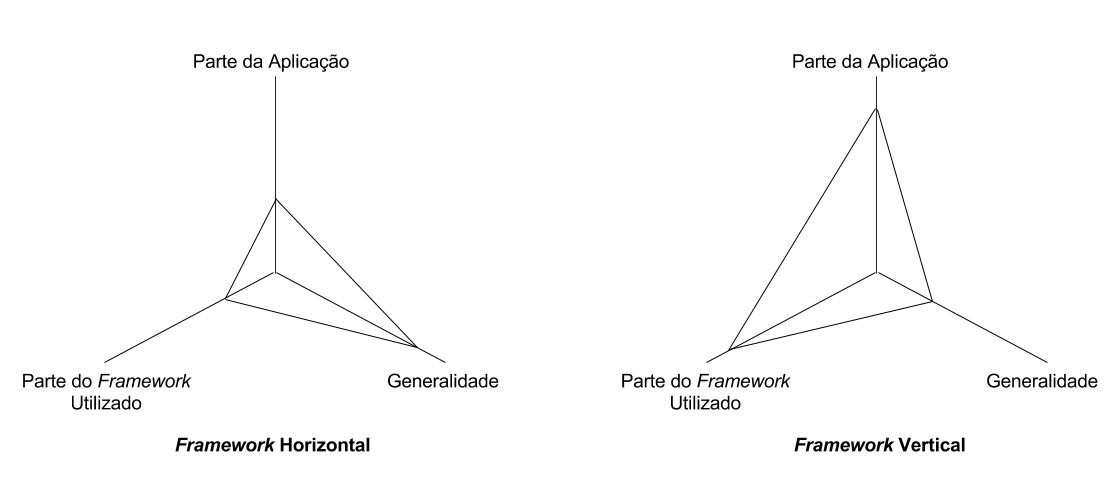
\includegraphics[width=\textwidth]{figuras/frameworkhorizontalvertical.png}
    \caption{Comparativo entre \textit{Framework} Horizontal e Vertical}
    \label{fig:frameworkhorizontalvertical}
  \end{figure}
\par
\begin{description}
\item[Framework de Horizontal:] é conhecido também como \textit{framework} de aplicação. O conhecimento embutido é passível de ser utilizado em uma grande variedade de aplicações, pois o seu foco é na generalização. Isso permite que o \textit{framework} possa ser utilizado em uma grande gama de aplicações, mas a parte do problema que ele resolve é menor \cite{barretoJunior2006}.
\item[Framework de Vertical:] também conhecido como \textit{framework} de domínio. O conhecimento encapsulado nesse tipo de \textit{framework} é mais específico a um domínio particular, o que confere ao \textit{framework} uma capacidade de dar maior suporte e, portanto, maior participação no desenvolvimento da aplicação. Porém, não permite a reutilização em uma diversidade de aplicações, na medida em que o domínio é específico. \cite{barretoJunior2006}.
\end{description}

\section{Geração e Automação de Testes}
A produção de testes de software é uma atividade que vem ganhando foco no desenvolvimento de aplicações. A qualidade do produto, ou serviço, resultante de projetos de software é um fator considerado essencial \cite{barbosaEtAl2009}. Testes de unidade são uma categoria de testes de software cujo objetivo e identificar os defeitos no código-fonte, o mais cedo possível. Isso implica que o desenvolvimento desse tipo de teste ocorra em paralelo com o desenvolvimento do software. No entanto, é comum que haja a defasagem entre a produção de testes e de código-fonte do software \cite{fantinatoEtAl2004}. Essa falta de sincronia ocorre por diversos fatores, dentre eles a falta de tempo e de qualificação técnica dos envolvidos \cite{fantinatoEtAl2004}.
\par
\indent Nesse contexto, o uso de ferramentas, e outras abordagens de automação de testes de software vem se tornando um medida bem vista para amenizar o problema \cite{fantinatoEtAl2004}. Em essência, a automação de testes de software é a prática de criar, normalmente via \textit{scripts}, meios do computador executar a tarefa de testar o código. Tendo isso em vista, as atividades de teste consideradas para automação são a geração de testes e execução \cite{fantinatoEtAl2004}.

\subsection{Técnicas de Geração e Automação de Teste}
Há diversas técnicas para automação da geração de testes. As principais técnicas são: \textbf{\textit{record/Playback}}, \textbf{\textit{script programming}}, \textbf{\textit{data-driven}} e \textbf{\textit{keyword-driven}} \cite{fantinatoEtAl2004}.
\subsubsection{\textit{Record/Playback}}
Em essência, a técnica de \textit{Record/Playback} consiste em repetir, de forma automática, um teste executado sobre a interface gráfica. Grava-se as ações produzidas pelo usuário e transcreve-se para um \textit{script}. A partir desse \textit{script} pode-se repetir as ações do usuário sempre que necessário. Assim, testa-se a aplicação utilizando-se as ações anteriormente bem sucedidas. Caso alguma das ações tenha insucesso, significa que algo foi quebrado. Os \textit{scripts} armazenam não apenas o procedimento de teste, mas também os dados utilizados pelo usuário para a execução deles \cite{kent2007}.
\par
\indent Como vantagens relativas ao \textit{Record/Playback}, pode-se citar a sua praticidade. No entanto, a quantidade de desvantagens é alta. Ao lidar-se com um número grande de casos de teste essa técnica mostra dificuldades relacionadas ao custo e complexidade de manutenção. Além disso, traz uma inerente sensibilidade a mudanças do software. O fato de ser específico a uma determinada interface também inviabiliza a reutilização dos testes \cite{fantinatoEtAl2004}.
\subsubsection{\textit{Script programming}}
Essa técnica é um melhoramento da técnica de \textit{Record/Playback}. Possui a mesma dinâmica de gravar as ações executadas por um usuário para, a partir de um \textit{script}, repetí-las. Diferencia-se pelo fato de alterar os \textit{scripts} originais de teste, inserindo novos comportamentos ao teste. Dessa forma, pode-se manter uma cópia do \textit{script} original e fazer diversas cópias que contemplem ações não executadas \cite{kent2007}.
\par
\indent Traz taxas maiores de manutenabilidade e reutilização que a \textit{Record/Playback}, como vantagens. Entretanto, ainda possui a problemática de gerar grandes quantidades de \textit{scripts} \cite{fantinatoEtAl2004}.
\subsubsection{\textit{Data-driven}}
Também conhecida como técnica orientada a dados. Nessa abordagem, que é um aprimoramento da técnica de \textit{script programming}, dá-se foco maior aos dados de teste utilizados em cada \textit{script}. Extrai-se esses dados dos \textit{scripts}, mantendo-os armazenados em outro arquivo. Assim, deixa apenas os procedimentos - lógica de execução - e as ações de teste escritos nos \textit{scripts}. Dessa maneira, os \textit{scripts} devem acessar os arquivos contendo os dados de teste para que haja a execução correta dos testes \cite{kent2007}.
\par
\indent Isto posto, observar-se algumas vantagens do uso dessa técnica: maior abstração dos testes, permitindo que haja o trabalho tanto do projetista de testes quanto do implementador, sem que haja preocupação de um nível de abstração com o outro. Enquanto o projetista visa a seleção dos melhores dados para o teste, o implementador prepara os \textit{scripts}. A facilidade em generalizar os \textit{scripts} e alterar os dados de teste pode ser vista como outra como outra vantagem dessa técnica. Permite maior reutilizaçã e manutenabilidade dos \textit{scripts} \cite{fantinatoEtAl2004}.
\subsubsection{\textit{Keyword-driven}}
Por meio dessa técnica pretende-se a extração da lógica (os procedimentos), de teste dos \textit{scripts}, e mantendo-os armazenados em outro arquivo. A partir do arquivo de procedimentos é que os \textit{scripts} retiram a lógica para efetuar as ações determinadas \cite{kent2007}.
\par
\indent Essa abordagem facilita a adição, remoção ou a alteração dos passos de execução de algum teste \cite{fantinatoEtAl2004}.











% Resumo do Capítulo